\chapter{LS59}
\label{cap:progetto3}

\section{Descrizione del Caso Studio}
\label{sec:paletta_descrizione}

Il terzo caso studio riguarda una \textbf{paletta di turbina con profilo LS59}, un profilo
transsonico tipico degli stadi di alta pressione dei turboventilatori. Il dominio
computazionale rappresenta un \emph{canale di cascata} (o \emph{cascade tunnel}): una
configurazione periodica in cui si simula il comportamento di una singola paletta
all'interno di una schiera infinita di profili identici, sfruttando la periodicità del
campo di moto per ridurre il dominio alla sola intercella.

La geometria è definita dal profilo LS59 che occupa la sezione centrale del canale, con
le condizioni di ingresso imposte con angolo di attacco $\alpha = 30°$ rispetto all'asse
orizzontale e numero di Mach $M_{\rm in} = 0.5$ (regime transonico basso). La pressione
statica di uscita $p_{\rm out} = 0.4124$ è ricavata dalle relazioni isentropiche per le
condizioni operative della paletta.

\section{Condizioni di Inlet e Outlet}

\begin{table}[h!]
\centering
\begin{tabular}{|l|l|l|}
\hline
 & \textbf{Inlet} & \textbf{Outlet} \\ \hline
\textbf{$T^\circ$} & 1 & - \\ \hline
\textbf{$p^\circ$} & 1 & - \\ \hline
\textbf{p} & - & 0.4124 \\ \hline
\textbf{M} & 0.5 & - \\ \hline
\textbf{Alpha} & $30^\circ$ & - \\ \hline
\end{tabular}
\caption{Condizioni di Inlet e Outlet - LS59}
\label{tab:ls59_conditions}
\end{table}

\section{Angolo di Attacco e Deflessione -- Considerazioni Teoriche}
\label{sec:paletta_angoli}

Un aspetto fondamentale nella simulazione di pale di turbina riguarda la corretta
interpretazione dell'angolo di attacco e della deflessione del flusso, grandezze che
influenzano direttamente le perdite di profilo e l'efficienza dello stadio.

\paragraph{Angolo di attacco.}
L'angolo di attacco $\alpha = 30°$ rappresenta l'angolo tra il vettore velocità in ingresso
e l'asse di riferimento del canale (asse $x$ orizzontale). Nelle cascate di turbina, a
differenza dei profili alari isolati, l'angolo di attacco è definito rispetto alla direzione
nominale di ingresso della schiera, non alla corda del profilo. Pertanto, piccole variazioni
di $\alpha$ rispetto al valore di progetto producono effetti di incidenza che si manifestano
principalmente sulla distribuzione di pressione intorno al bordo di attacco e sulla posizione
del punto di ristagno.

\paragraph{Deflessione del flusso.}
La deflessione $\Delta\beta = \beta_{\rm in} - \beta_{\rm out}$ (differenza tra angolo di
ingresso e angolo di uscita misurati rispetto all'asse tangenziale) è la grandezza che
quantifica il lavoro estratto dalla paletta. Per il profilo LS59, la deflessione di progetto
è tale da garantire un campo di pressione uniforme sull'intradosso e un'accelerazione
controllata sull'estradosso, minimizzando le perdite per separazione dello strato limite.

\paragraph{Effetto dell'angolo di attacco sulle prestazioni.}
Nella paletta di turbina LS59, variazioni dell'angolo di attacco rispetto al valore nominale
($\alpha = 30°$) hanno i seguenti effetti:
\begin{itemize}
  \item \textbf{Incidenza positiva} ($\alpha > 30°$): carico aerodinamico maggiore sul
    bordo di attacco, rischio di separazione precoce sull'intradosso e aumento delle perdite
    di profilo.
  \item \textbf{Incidenza negativa} ($\alpha < 30°$): sottocarico del bordo di attacco,
    possibile separazione sull'estradosso con conseguente riduzione della deflessione
    effettiva e calo dell'efficienza di palettatura.
  \item \textbf{Valore di progetto} ($\alpha = 30°$): distribuzione di carico ottimale,
    minime perdite di profilo e comportamento isentropico prossimo a quello teorico.
\end{itemize}
In un modello di Eulero (flusso non viscoso), tali effetti di separazione non sono
direttamente simulabili; tuttavia, il campo di pressione risultante fornisce informazioni
preziose sul \emph{carico del profilo} (integrale della differenza di pressione tra
intradosso ed estradosso) e sulla distribuzione di velocità, che possono essere confrontate
con i dati sperimentali per validare il codice numerico e identificare zone critiche dove
gli effetti viscosi diventano rilevanti.

\section{Mesh di Calcolo}
\label{sec:paletta_mesh}

Per il profilo LS59 \textbf{l'analisi di convergenza di griglia non viene ripetuta}: come
previsto dalla traccia, tale studio è condotto sul solo caso della presa a doppia rampa
(Cap.~\ref{cap:doppia_presa}). Per la paletta si adotta quindi direttamente una
\textbf{griglia sufficientemente fine}, già in regime di convergenza, generata con una
lunghezza caratteristica $l_c = 0.01$. Questo valore è abbastanza piccolo da risolvere
adeguatamente i gradienti attorno al profilo --- in particolare in corrispondenza del bordo di
attacco e di fuga, dove la curvatura è massima --- senza appesantire eccessivamente il calcolo.

\begin{figure}[H]
  \centering
  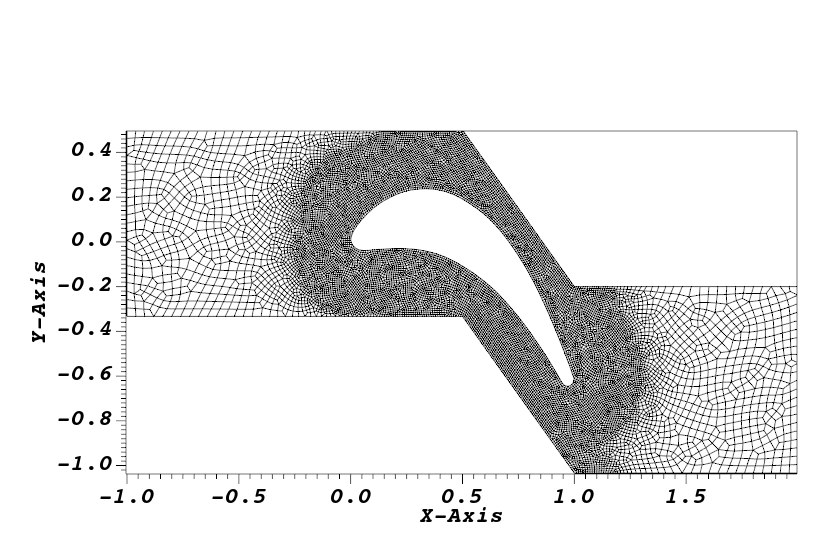
\includegraphics[width=0.85\textwidth]{../Images/Eulero_LS59_mesh.jpg}
  \caption{Mesh non strutturata (a prevalenza di quadrilateri) della singola intercella
           periodica della schiera LS59, generata con lunghezza caratteristica $l_c = 0.01$.
           Si nota l'infittimento spontaneo nella fascia che avvolge il profilo e nel canale
           inter-pala, mentre le regioni di monte e di valle, dove il campo è pressoché
           uniforme, presentano celle più rade.}
  \label{fig:eulero_ls59_mesh}
\end{figure}

Essendo la mesh già adeguata, non si riportano confronti tra livelli di griglia: quella di
Figura~\ref{fig:eulero_ls59_mesh} è la griglia effettivamente impiegata per tutti i risultati
Euler presentati nel seguito (schema di Roe).

\section{Confronto con Dati Sperimentali e Analisi con ANSYS Fluent}
\label{sec:paletta_confronto}

La distribuzione di pressione (o equivalentemente il coefficiente di pressione $C_p$)
attorno al profilo LS59 costituisce il principale termine di confronto tra il codice
numerico, ANSYS Fluent e i dati sperimentali di letteratura per questo tipo di paletta.

Per il confronto si estrae la pressione statica adimensionale $P_w/P^\circ$ nelle celle
di bordo che definiscono il profilo (tag di parete solida), separando l'intradosso
dall'estradosso tramite la coordinata $y$ delle celle, e si confronta con i dati
sperimentali disponibili.

\begin{figure}[H]
  \centering
  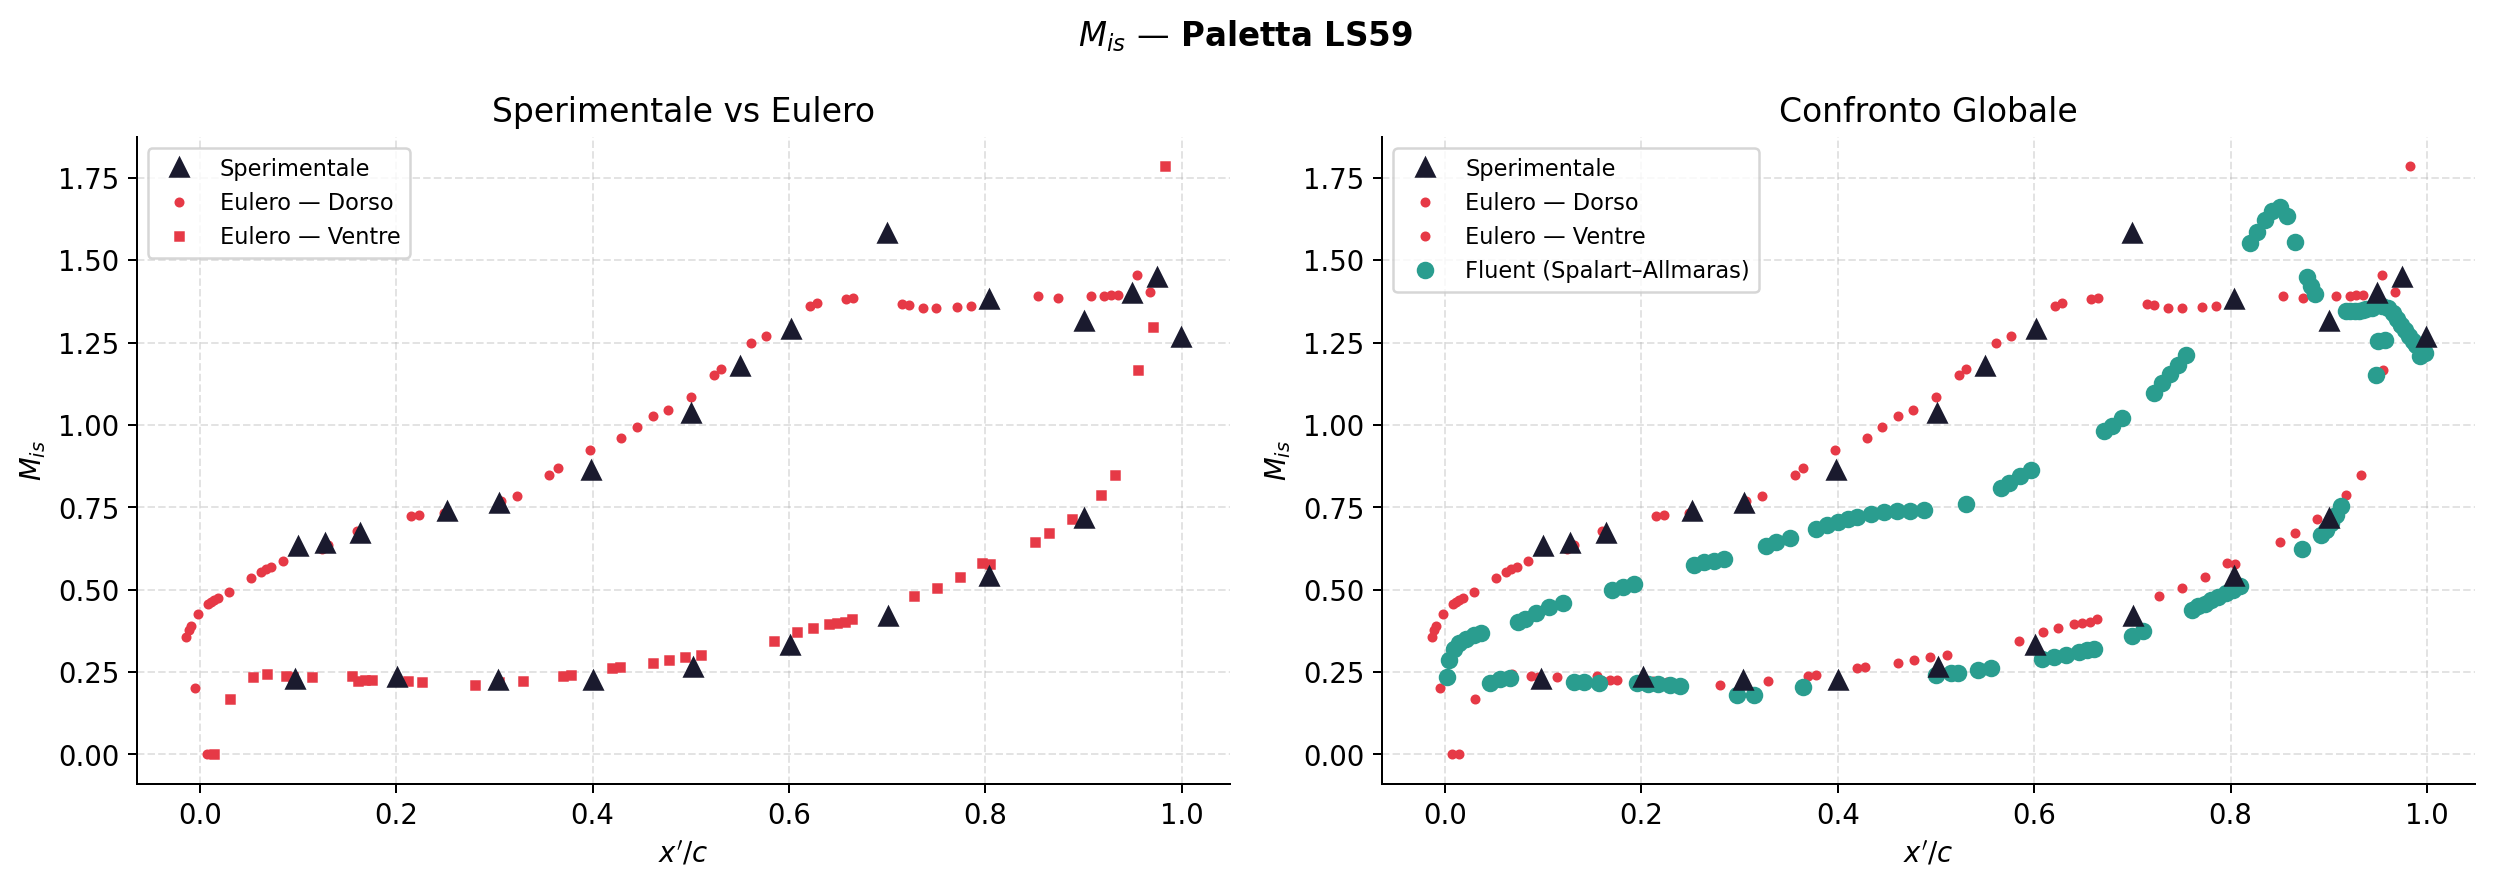
\includegraphics[width=0.85\textwidth]{../Images/confronto_Mis_LS59}
  \caption{Distribuzione di pressione adimensionale $P_w/P^\circ$ attorno al profilo LS59:
           confronto tra i dati sperimentali, la soluzione Euler con schema di Roe (codice
           sviluppato), la soluzione Euler--CFD (ANSYS Fluent inviscido) e il modello RANS
           Spalart--Allmaras (ANSYS Fluent viscoso).
           I modelli inviscidi concordano bene con i dati sperimentali sull'intradosso,
           dove il flusso rimane attaccato; le discrepanze sull'estradosso, in prossimità
           del bordo di uscita, sono attribuibili agli effetti viscosi e alla separazione
           dello strato limite non modellata dalle equazioni di Eulero.}
  \label{fig:confronto_Mis_LS59}
\end{figure}

% L'analisi ANSYS Fluent completa (mesh, y+, campi Mach/pressione, profili di
% strato limite e confronto con dati sperimentali) è trattata nel
% Capitolo~\ref{cap:fluent} dedicato, al fine di evitare duplicazione.

\section{Campi di Mach, Pressione e Temperatura}
\label{sec:paletta_campi}

Si analizzano di seguito i campi di pressione, numero di Mach e temperatura ottenuti con il
codice Euler sviluppato (schema di Roe). Tutte le grandezze sono \textbf{adimensionali},
riferite alle condizioni totali di ingresso ($P^\circ_{\rm in} = 1$, $T^\circ_{\rm in} = 1$);
in particolare la pressione mostrata è $P/P^\circ_{\rm in}$ e la temperatura $T/T^\circ_{\rm in}$.
I tre campi, letti in modo incrociato, risultano \textbf{mutuamente coerenti} con le relazioni
isentropiche, il che costituisce di per sé una prima validazione del codice.

\subsection{Campo di Pressione}
\label{sec:paletta_pressione}

\begin{figure}[H]
  \centering
  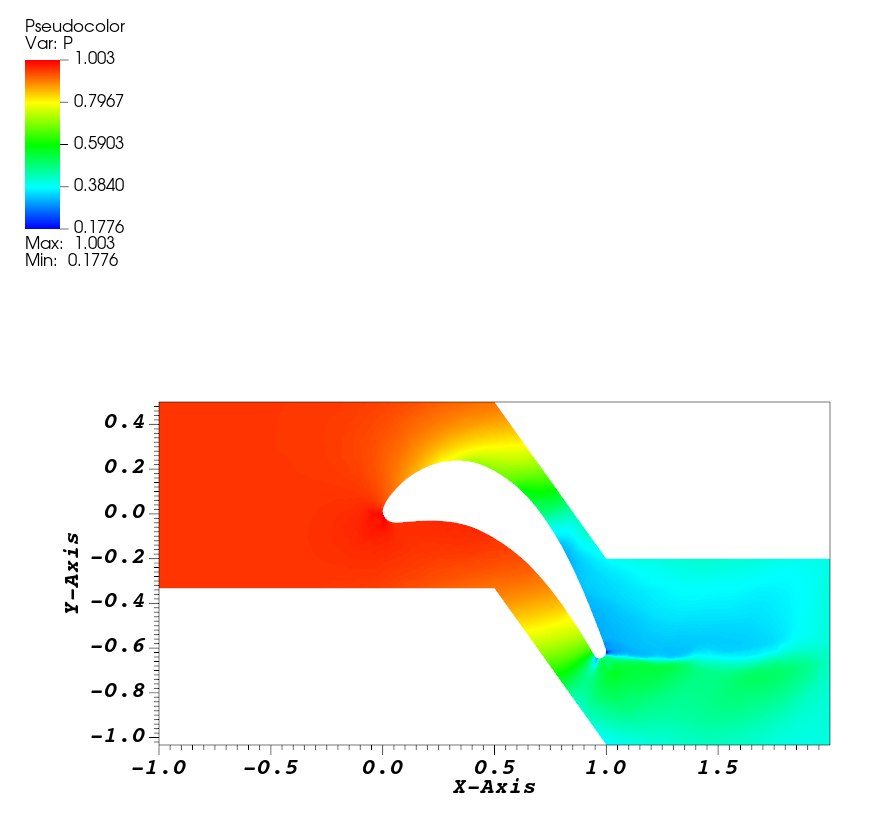
\includegraphics[width=0.85\textwidth]{../Images/Eulero_LS59_pressione.jpg}
  \caption{Campo di pressione adimensionale $P/P^\circ_{\rm in}$ attorno al profilo LS59
           (codice Euler, schema di Roe). Scala: $P_{\max} = 1.003$ (punto di ristagno),
           $P_{\min} = 0.178$. A monte il campo è uniforme; sul dorso si sviluppa una marcata
           depressione, mentre a valle la pressione si assesta sul valore di uscita
           ($\approx 0.41$).}
  \label{fig:eulero_ls59_pressione}
\end{figure}

\paragraph{Uniformità a monte.}
Come atteso, a monte del profilo il campo di pressione è \textbf{uniforme}: la corrente non ha
ancora "sentito" la presenza della paletta. Il valore numerico letto dal grafico in questa
regione (circa $0.84$) coincide con la \textbf{pressione statica di freestream} associata al
Mach di ingresso, come verificato di seguito. A valle, la pressione si porta sul valore di
scarico imposto ($P_{\rm out} = 0.4124$), coerente con la fascia ciano della scala.

\paragraph{Pressione attesa al punto di ristagno.}
Il dubbio sul perché la differenza tra ristagno e monte appaia "piccola" si chiarisce con il
calcolo. Le condizioni di ingresso sono $P^\circ_{\rm in} = 1$ (pressione \emph{totale},
adimensionale) e $M_{\rm in} = 0.5$. La \textbf{pressione statica a monte} si ricava dalla
relazione isentropica:
\begin{equation}
  \frac{P_\infty}{P^\circ_{\rm in}}
  = \left(1 + \frac{\gamma-1}{2}M_\infty^2\right)^{-\frac{\gamma}{\gamma-1}}
  = \left(1 + 0.2\cdot 0.5^2\right)^{-3.5}
  = (1.05)^{-3.5} \approx 0.843
  \label{eq:p_statica_monte}
\end{equation}
Al \textbf{punto di ristagno} la corrente si arresta ($M = 0$): per definizione tutta l'energia
cinetica si converte in pressione, quindi la pressione statica eguaglia quella totale. Poiché il
flusso è isentropico (Euler subsonico, privo di urti) la pressione totale si \emph{conserva} ed è
pari a quella di ingresso:
\begin{equation}
  P_{\rm rist} = P^\circ_{\rm in} = 1.000
\end{equation}
La differenza attesa tra ristagno e monte è quindi:
\begin{equation}
  \Delta P = P_{\rm rist} - P_\infty \approx 1.000 - 0.843 = 0.157 \quad (\approx 16\%)
\end{equation}
\textbf{La differenza è dunque tutt'altro che trascurabile} (circa il 16\%). Il valore massimo
letto sul campo, $P_{\max} = 1.003$, conferma quasi esattamente la previsione $P_{\rm rist} = 1.0$
(lo scarto di $+0.3\%$ è un piccolo \emph{overshoot} numerico, si veda
Sez.~\ref{sec:paletta_roe}). L'impressione di una differenza "piccola" nasce unicamente dalla
\textbf{scala cromatica}: l'intervallo $0.84 \div 1.00$ ricade tutto nella parte alta (toni caldi
arancio--rosso) della color-bar, perciò la variazione, pur reale e pari al 16\%, appare compressa
in tonalità simili. La controprova viene dal campo di temperatura (Sez.~\ref{sec:paletta_temp}),
dove a monte $T_\infty/T^\circ = (1.05)^{-1} \approx 0.952$ in accordo con il valore arancione
osservato, e al ristagno $T \to T^\circ = 1.0$.

\paragraph{Depressione sul dorso: geometria/deflessione o incidenza?}
La pressione scende sul \textbf{dorso} (estradosso) molto più di quanto non faccia sul
\textbf{ventre} (intradosso), come atteso. Il meccanismo \emph{primario} è la
\textbf{geometria del profilo e la deflessione} che esso impone alla corrente: per deviare il
flusso, il lato convesso (dorso) deve \textbf{accelerare} il fluido (le linee di corrente si
infittiscono e curvano), il che per Bernoulli/relazioni isentropiche comporta una
\textbf{caduta di pressione}; il lato concavo (ventre) al contrario \textbf{decelera} la corrente
e la pressione resta alta. È questa differenza intradosso--estradosso a generare il
\textbf{carico} della paletta e quindi il lavoro scambiato. L'\textbf{angolo di attacco/incidenza}
($\alpha = 30^\circ$, discusso in Sez.~\ref{sec:paletta_angoli}) ha invece un ruolo
\emph{secondario di modulazione}: fissa la posizione del punto di ristagno e l'entità del picco di
depressione vicino al bordo di attacco. Al valore di progetto il carico è distribuito in modo
ottimale; a incidenza fuori progetto il picco si sposta e si accentua, ma la natura della
depressione sul dorso rimane dettata dalla \textbf{curvatura e deflessione}. In sintesi:
\textbf{geometria e deflessione come causa principale, incidenza come modulatore}.

\paragraph{La linea isobara "ad archetto" sul dorso.}
La linea gialla che si osserva sul dorso è, correttamente, una \textbf{isobara} (linea a pressione
costante). La sua interpretazione discende dall'equilibrio dei gradienti di pressione in un flusso
\textbf{curvo}: in direzione normale alle linee di corrente vale
\begin{equation}
  \frac{\partial P}{\partial n} = \rho\,\frac{V^2}{R}
\end{equation}
ovvero la pressione cresce allontanandosi dalla parete convessa (raggio di curvatura $R$). Vicino
alla superficie del dorso la pressione è minima e \textbf{aumenta spostandosi verso il cuore del
canale}; quando le linee di corrente tornano \emph{rettilinee} (zona centrale del canale
inter-pala) il gradiente normale si annulla e la pressione diventa \textbf{uniforme}. L'isobara
gialla segna proprio il \textbf{confine} tra la regione a flusso curvo (adiacente al profilo, dove
$P$ varia rapidamente) e il nucleo a flusso quasi rettilineo (dove $P$ è costante): poiché segue
la curvatura del dorso, assume la caratteristica forma \textbf{ad arco}. Lo stesso fenomeno è
visibile, più debolmente, in altre zone curve del campo.

\paragraph{C'è separazione, scia o turbolenza?}
È un punto importante: il modello è di \textbf{Eulero}, cioè \textbf{non viscoso}. Di conseguenza
\textbf{non possono esistere né separazione di strato limite né turbolenza}, che sono fenomeni
intrinsecamente viscosi. La regione dalla forma "strana" delle isobare sul dorso, in coda al
profilo, \emph{non} è quindi una separazione turbolenta. Si tratta piuttosto di una
\textbf{ricompressione/scia inviscida} in prossimità del bordo di fuga (dove le correnti di dorso e
ventre si ricongiungono) ed eventualmente di una \textbf{debole onda di compressione} nella zona
transonica del dorso (si veda il campo di Mach). Una vera separazione comparirebbe soltanto nelle
simulazioni \textbf{viscose} (RANS con Spalart--Allmaras, Cap.~\ref{cap:fluent}), non in questo
campo Euler.

\subsection{Campo di Mach}
\label{sec:paletta_mach}

\begin{figure}[H]
  \centering
  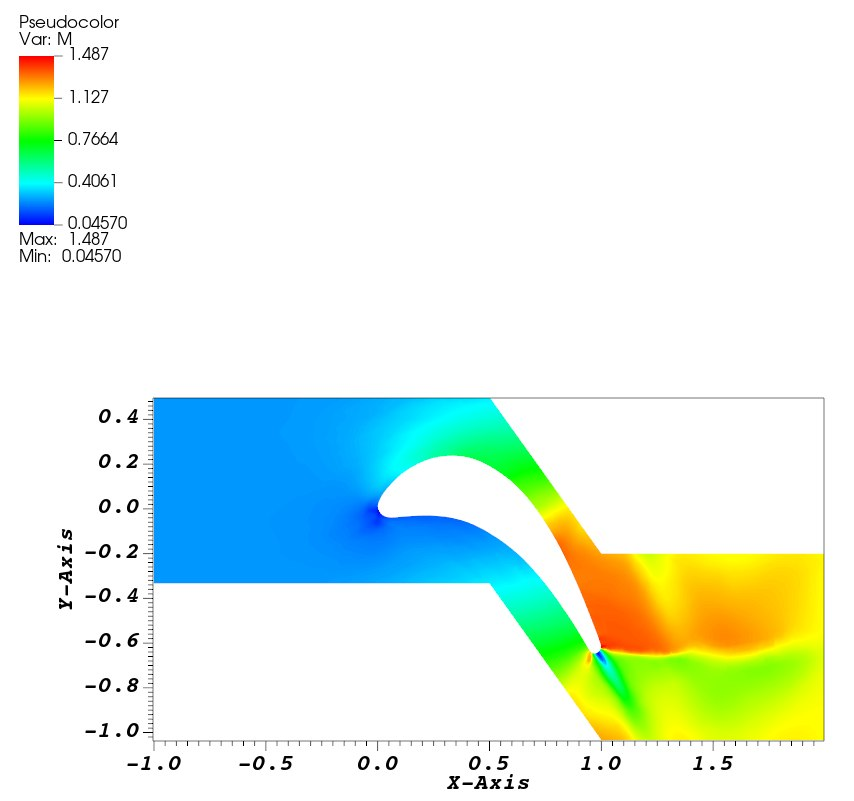
\includegraphics[width=0.85\textwidth]{../Images/Eulero_LS59_mach.jpg}
  \caption{Campo del numero di Mach attorno al profilo LS59 (codice Euler, schema di Roe).
           Scala: $M_{\max} = 1.487$, $M_{\min} = 0.046$. A monte $M \approx 0.5$; al bordo di
           attacco si osserva il punto di ristagno ($M \to 0$); sul dorso la corrente accelera
           fino a divenire \textbf{supersonica} ($M > 1$) nella parte posteriore del canale.}
  \label{fig:eulero_ls59_mach}
\end{figure}

\paragraph{Aspetti salienti.}
Il campo di Mach riassume la fisica della schiera:
\begin{itemize}
  \item \textbf{Ingresso uniforme} a $M_\infty \approx 0.5$ (fascia ciano a monte), coerente con
    la condizione al contorno imposta.
  \item \textbf{Punto di ristagno} al bordo di attacco, dove $M \to 0$ (macchia blu, $M_{\min}
    \approx 0.05$): qui la corrente si arresta, in accordo con il picco di pressione e di
    temperatura negli altri due campi.
  \item \textbf{Accelerazione sul dorso}: la corrente accelera fortemente sull'estradosso fino a
    raggiungere e superare $M = 1$, con un \textbf{cuscinetto supersonico} ($M$ fino a $\sim 1.3$--$1.5$)
    nella parte posteriore del canale. La LS59 è infatti una paletta \textbf{transonica}: l'uscita
    è supersonica (coerente con il $M_{\rm out}$ di progetto e con la $P_{\rm out}$ imposta).
  \item \textbf{Ventre} a Mach più contenuto (la corrente decelera), confermando l'asimmetria di
    carico dorso/ventre.
  \item \textbf{Scia al bordo di fuga}: a valle del trailing edge si osserva una regione a Mach
    ridotto, traccia della scia inviscida e del ricongiungimento delle due correnti.
\end{itemize}

\paragraph{Gli "spike" al bordo di attacco e al bordo di fuga.}
I piccoli picchi localizzati di Mach in corrispondenza dei bordi hanno origine in parte fisica e
in parte numerica:
\begin{itemize}
  \item \textbf{Bordo di attacco}: subito a valle del punto di ristagno la corrente
    \textbf{accelera bruscamente} contornando la forte curvatura del naso, generando un
    \emph{picco di sovravelocità} (leading-edge suction peak). È un effetto fisico reale, ma
    \textbf{amplificato} dalla risoluzione di griglia in una zona ad altissima curvatura e dal
    comportamento dello schema di Roe in prossimità dei punti di ristagno.
  \item \textbf{Bordo di fuga}: il trailing edge, in un calcolo \textbf{inviscido}, è un
    \textbf{punto singolare} (la condizione di Kutta non è imposta naturalmente). Il
    ricongiungimento delle correnti e la geometria a spigolo producono un picco locale di Mach,
    in larga parte di natura \textbf{numerica}.
\end{itemize}

\subsection{Campo di Temperatura}
\label{sec:paletta_temp}

\begin{figure}[H]
  \centering
  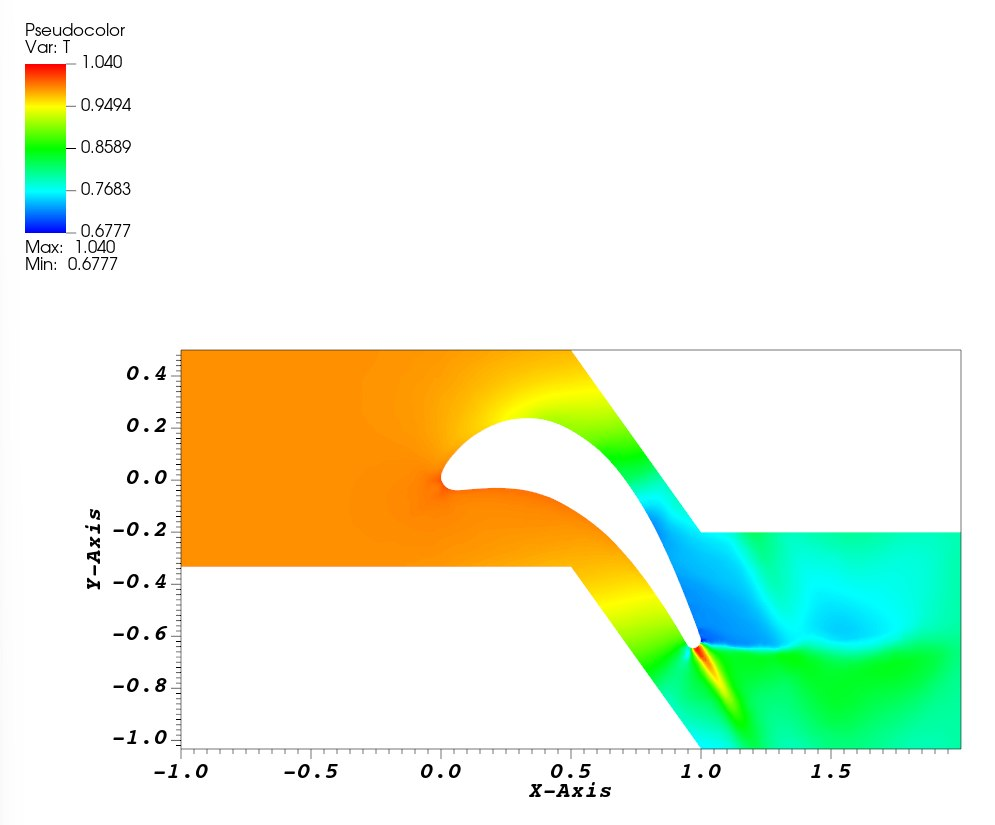
\includegraphics[width=0.85\textwidth]{../Images/Eulero_LS59_temperatura.jpg}
  \caption{Campo di temperatura adimensionale $T/T^\circ_{\rm in}$ attorno al profilo LS59
           (codice Euler, schema di Roe). Scala: $T_{\max} = 1.040$, $T_{\min} = 0.678$.
           Si noti la marcata \textbf{spike di temperatura} in uscita dal bordo di fuga.}
  \label{fig:eulero_ls59_temperatura}
\end{figure}

\paragraph{Andamento generale.}
Il campo di temperatura è il "negativo" di quello di Mach, come imposto dalla relazione
isentropica $T/T^\circ = (1 + \frac{\gamma-1}{2}M^2)^{-1}$: dove la corrente accelera, la
temperatura \textbf{cala}. A monte $T_\infty \approx 0.95$ (coerente con $M = 0.5$), al ristagno
$T \to T^\circ = 1.0$, e sul dorso supersonico la temperatura scende fino al minimo
$T_{\min} \approx 0.68$ (in accordo con $M \approx 1.5$).

\paragraph{La spike al bordo di fuga.}
La sottile lingua calda che esce dal bordo di fuga è un \textbf{artefatto numerico} legato alla
singolarità inviscida del trailing edge. L'indizio decisivo è che il \textbf{massimo del campo
vale $T_{\max} = 1.040 > T^\circ = 1.0$}: poiché la temperatura totale è il limite \emph{superiore}
fisicamente raggiungibile dalla temperatura statica (la si ottiene solo arrestando isentropicamente
la corrente), \textbf{un valore superiore a $T^\circ$ è impossibile} e segnala inequivocabilmente un
\emph{overshoot} numerico. La spike è \textbf{particolarmente accentuata} perché in quel punto
concorrono più fattori: (i) la \textbf{singolarità geometrica} dello spigolo di uscita; (ii) il
\textbf{ricongiungimento} di due correnti con stato leggermente diverso (piccola differenza di
entropia tra dorso e ventre, che inviscidamente si concentra in una linea di contatto); (iii) la
\textbf{bassa densità} locale del gas espanso, che amplifica la sensibilità della temperatura agli
errori; (iv) la \textbf{concentrazione dell'entropia numerica} prodotta dallo schema proprio nella
zona del trailing edge. In un calcolo \textbf{viscoso} la stessa zona presenterebbe una scia
regolare e diffusa, senza il picco puntuale.

\subsection{Artefatti Numerici dello Schema di Roe}
\label{sec:paletta_roe}

Diversi dettagli dei campi sono riconducibili al comportamento dello \textbf{schema di Roe}, molto
poco dissipativo e quindi accurato ma soggetto ad alcune anomalie note in punti critici:
\begin{itemize}
  \item \textbf{Overshoot al ristagno}: il valore $P_{\max} = 1.003 > 1.0$ (e analogamente
    $T_{\max} = 1.040 > 1.0$) è un piccolo sovra-tiro non fisico tipico dei punti di ristagno,
    dove la bassa dissipazione di Roe non smorza del tutto le oscillazioni locali.
  \item \textbf{Anomalie ai bordi di attacco e di fuga}: gli spike di Mach e temperatura descritti
    sopra sono coerenti con le \emph{stagnation-point anomalies} dello schema di Roe, accentuate
    nelle zone di forte curvatura e nelle singolarità inviscide (trailing edge).
  \item \textbf{Punti sonici}: nell'attraversamento $M = 1$ sul dorso lo schema di Roe richiede una
    \emph{entropy fix} (di Harten, già adottata nel codice) per evitare espansioni non fisiche; sue
    eventuali tracce sarebbero localizzate proprio nella zona transonica del dorso.
\end{itemize}
Tali artefatti sono \textbf{locali e di entità contenuta} e non inficiano la qualità complessiva
della soluzione, ma è corretto segnalarli per una lettura critica dei campi.

\subsection{Osservazioni Conclusive}
\label{sec:paletta_oss}

\begin{itemize}
  \item I tre campi sono \textbf{reciprocamente coerenti} con le relazioni isentropiche
    (verificato ai punti di monte, di ristagno e nella zona supersonica del dorso): ciò
    \textbf{valida} il corretto funzionamento del solutore Euler.
  \item La paletta opera in regime \textbf{transonico}: ingresso subsonico ($M = 0.5$), uscita
    supersonica, con un cuscinetto $M > 1$ sul dorso. Questo giustifica anche la scelta delle
    condizioni al contorno (pressione statica imposta all'outlet subsonico-equivalente / uscita).
  \item Gli scostamenti rispetto alla realtà fisica (assenza di scia viscosa regolare, spike al
    bordo di fuga, mancata separazione) sono il \textbf{prezzo del modello inviscido} e vengono
    recuperati nelle simulazioni RANS del Cap.~\ref{cap:fluent}.
  \item L'\textbf{entropia numerica} si concentra, come atteso, nelle singolarità (bordo di fuga):
    è la principale sorgente di discrepanza con il confronto sperimentale di
    Sez.~\ref{sec:paletta_confronto}.
\end{itemize}
